\documentclass[11pt]{article}

\usepackage[a4paper,margin=2.6cm]{geometry}
\usepackage{amsmath,amssymb,amsthm,mathtools}
\usepackage{booktabs}
\usepackage{graphicx}
\usepackage{xcolor}
\usepackage{hyperref}
\usepackage{enumitem}
\usepackage{caption}
\captionsetup{font=small,labelfont=bf}

\hypersetup{colorlinks=true,linkcolor=blue!55!black,urlcolor=blue!55!black,
            pdftitle={Stoichiometry of a saturated fluorite nanoparticle}}

\theoremstyle{plain}
\newtheorem{theorem}{Theorem}[section]
\newtheorem{proposition}[theorem]{Proposition}
\theoremstyle{definition}
\newtheorem{definition}[theorem]{Definition}
\newtheorem{example}[theorem]{Example}
\theoremstyle{remark}
\newtheorem*{remark}{Remark}

\newcommand{\Z}{\mathbb{Z}}
\newcommand{\NA}{N_{\!A}}
\newcommand{\NB}{N_{\!B}}
\newcommand{\eps}{\varepsilon}
\DeclareMathOperator{\ceil}{ceil}

\title{Stoichiometry of a saturated fluorite nanoparticle\\[2pt]
\large Exact lattice counts for axis-aligned nanocubes and boxes}
\author{}
\date{}

\begin{document}
\maketitle

\begin{abstract}
We consider a fluorite ($AB_2$) nanoparticle in the idealised limit where every
cation~$A$, including those at the surface, retains its full eightfold
coordination by anions~$B$.  In this model the anions form a simple-cubic
lattice and the cations occupy the body centres of one checkerboard colour of
the anion cubes.  The stoichiometry is therefore an exact finite
lattice-counting problem.  We prove a bond-counting identity showing that every
finite saturated particle is $B$-rich, show by example that the ratio is not a
function of $\NA$ alone, and derive closed forms for every axis-aligned
$a\times b\times c$ box.  The associated $n\times n\times n$ nanocube sequences
are elementary parity-modulated polynomials; the full $B$-count and $B$-excess
sequences currently have no direct OEIS match and are natural, though modest,
catalogue candidates.
\end{abstract}

\section{The fluorite structure, recast}

In the conventional cubic cell of fluorite CaF$_2$ (side~$a$), the cation~$A$
occupies the fcc positions and the anion~$B$ occupies all eight tetrahedral
holes.  The useful simplification is to read the structure from the anion side.

\begin{proposition}\label{prop:recast}
In fluorite, $B$ forms a simple-cubic lattice of spacing~$a/2$,
\[
B = \tfrac{a}{2}\Z^3 + \tfrac{a}{4}(1,1,1),
\]
and $A$ sits at the body centre of every second $B$-cube.  In $B$-lattice units,
indexing unit $B$-cubes by $(i,j,k)\in\Z^3$,
\[
A = \{(i+\tfrac12,j+\tfrac12,k+\tfrac12): i+j+k\text{ even}\}.
\]
Consequently $\mathrm{CN}(A)=8$ and $\mathrm{CN}(B)=4$ in the infinite bulk.
The number densities in these units are $\rho_A=1/2$ and $\rho_B=1$.
\end{proposition}

\begin{proof}
The eight tetrahedral holes are $(a/4)(\pm1,\pm1,\pm1)$; together with
translations by $a\Z^3$ they form $\tfrac{a}{2}\Z^3+(a/4)(1,1,1)$.  Shifting
the origin by $(a/4)(1,1,1)$ places the anions at the integer lattice.  The fcc
cation positions are then the body centres of exactly one checkerboard colour
of the unit cubes.  The coordination numbers are immediate from the cube-corner
incidence.
\end{proof}

\section{The saturation model}

\begin{definition}[saturated particle]
A particle is specified by a finite set~$S$ of $A$-sites.  Its $B$-set is
\[
B(S)=\bigcup_{A\in S}\{\text{the eight corner-$B$ sites of the $A$ cube}\}.
\]
Thus every selected cation, including a surface cation, keeps its full
eightfold $B$ shell.  Shared corner anions are counted once.
\end{definition}

Let $\NA=|S|$, $\NB=|B(S)|$, and let $d_B\in\{1,2,3,4\}$ be the number of
selected $A$-cubes incident on a given included $B$ site.

\begin{theorem}[bond-counting identity]\label{thm:bond}
For every finite saturated particle,
\[
\boxed{\;\NB-2\NA=\frac14\sum_{B\in B(S)}(4-d_B)\ge 0.\;}
\]
Equality is impossible for a nonempty finite particle, so every finite saturated
particle is strictly $B$-rich.
\end{theorem}

\begin{proof}
Counting $A$--$B$ incidences from the $A$ side gives $8\NA$.  Counting the same
incidences from the $B$ side gives $\sum_B d_B$.  Hence
\[
2\NA=\frac14\sum_B d_B,
\qquad
\NB-2\NA=\frac14\sum_B(4-d_B).
\]
Each summand is non-negative because a $B$ site has at most four adjacent
checkerboard $A$-cubes.  A finite particle must have boundary $B$ sites with
$d_B<4$.
\end{proof}

The excess $\NB-2\NA$ is therefore a direct measure of missing bulk neighbours
at the boundary.

\section{The ratio is not a function of the cation count alone}

\begin{proposition}[form-factor dependence]\label{prop:nonuniv}
Two saturated particles with the same $\NA$ can have different $\NB$.
\end{proposition}

\begin{example}
The $2\times2\times2$ axis-aligned cube has $\NA=4$ and $\NB=23$.  The
$4\times2\times1$ slab also has $\NA=4$, but it has $\NB=26$.  Thus the ratio is
$1{:}5.75$ in one case and $1{:}6.50$ in the other.
\end{example}

Consequently one should not expect a universal function $\NB=f(\NA)$.  A
well-defined sequence appears only after choosing a shape family and a placement
convention.

\section{Axis-aligned boxes}\label{sec:boxes}

The cleanest exact family is the axis-aligned box
$[0,a)\times[0,b)\times[0,c)$ of $B$-cubes, with the selected $A$-sites those
for which $i+j+k$ is even.

\begin{theorem}[box formula]\label{thm:box}
For positive integers $a,b,c$,
\[
\NA=\ceil\!\left(\frac{abc}{2}\right),
\qquad
\NB=(a+1)(b+1)(c+1)-U,
\]
where $U\in\{0,1,2,3,4\}$ is the number of enclosing-box vertices not incident
to any selected $A$-cube.  If $\eps=1$ when $a,b,c$ are all odd and $\eps=0$
otherwise, then
\[
\boxed{\;\NB-2\NA=(ab+ac+bc)+(a+b+c)+(1-U-\eps).\;}
\tag{1}\label{eq:box}
\]
\end{theorem}

\begin{proof}
The number of even-parity triples in the $a\times b\times c$ index box is
$\ceil(abc/2)$, giving $\NA$.  If all cube colours were present, the touched
$B$-vertices would be the full grid of size $(a+1)(b+1)(c+1)$.  With only one
checkerboard colour, the only possible omissions are enclosing-box vertices
whose unique incident in-box cube has odd parity; their count is $U$.  Therefore
$\NB=(a+1)(b+1)(c+1)-U$.  Subtracting $2\NA=abc+\eps$ and expanding gives
Eq.~\eqref{eq:box}.
\end{proof}

The three terms in Eq.~\eqref{eq:box} have a useful interpretation for this
axis-aligned family.  The leading term $ab+ac+bc$ is the sum of the three
coordinate projected areas of the box.  The next term $a+b+c$ is an edge-order
correction.  The final term is a bounded parity/corner correction.

For any fixed axis-aligned aspect ratio $(\alpha,\beta,\gamma)$ scaled by a
large parameter $m$, the excess is of order $m^2$ while $\NA$ is of order
$m^3$.  Thus
\[
\frac{\NB}{\NA}=2+c_{\alpha,\beta,\gamma}\NA^{-1/3}+o(\NA^{-1/3}),
\qquad
c_{\alpha,\beta,\gamma}=
\frac{\alpha\beta+\alpha\gamma+\beta\gamma}{(\alpha\beta\gamma/2)^{2/3}}.
\tag{2}\label{eq:box_asym}
\]
For the cube this gives $c=3\cdot2^{2/3}\approx4.762$.

\begin{remark}[scope]
Equation~\eqref{eq:box} is an exact axis-aligned box result, not a universal
surface theorem.  A tempting continuum argument would inflate a region by the
full cube $[-1/2,1/2]^3$, leading to a projected-area formula for arbitrary
orientations.  That argument ignores that the $A$ sites occupy only one
checkerboard colour.  Oblique and curved boundaries sample the checkerboard
adjacency differently, so no sphere, ellipsoid, or Wulff-shape claim is made
here.
\end{remark}

\section{Cubic-shell sequences and the OEIS}\label{sec:seq}

For the $n\times n\times n$ saturated cube, using the checkerboard phase that
contains the origin cube, Theorem~\ref{thm:box} gives
\[
\NA(n)=\ceil\!\left(\frac{n^3}{2}\right),
\qquad
\NB(n)=(n+1)^3-2\bigl(1+(-1)^n\bigr),
\]
and
\[
\NB(n)-2\NA(n)=3n(n+1)-\frac32\bigl(1+(-1)^n\bigr)
=
\begin{cases}
3n(n+1), & n\text{ odd},\\[2pt]
3(n^2+n-1), & n\text{ even}.
\end{cases}
\]

The phase convention matters for odd $n$: the opposite checkerboard colour in
the same enclosing cube has one fewer $A$ site and a different $B$ count.  The
choice above matches the $\ceil(n^3/2)$ convention of A036486.

\begin{table}[ht]\centering
\caption{Cubic-shell sequences and OEIS status.  Direct OEIS searches on
2026-06-25 returned no match for the candidate rows.}
\label{tab:seq}\small
\begin{tabular}{@{}lll@{}}
\toprule
sequence & first terms & OEIS \\
\midrule
$\NA$ (full) & 1, 4, 14, 32, 63, 108, 172, 256, \dots &
\href{https://oeis.org/A036486}{A036486} $\ceil(n^3/2)$ \\
$\NA$ odd shells & 1, 14, 63, 172, 365, 666, 1099, \dots &
\href{https://oeis.org/A050492}{A050492} thickened cubes \\
$\NB$ odd shells & 8, 64, 216, 512, 1000, 1728, \dots &
\href{https://oeis.org/A016743}{A016743} even cubes \\
excess odd shells & 6, 36, 90, 168, 270, 396, \dots &
\href{https://oeis.org/A152746}{A152746} $6\times$ hexagonal numbers \\
\midrule
$\NB$ (full) & 8, 23, 64, 121, 216, 339, 512, 725, \dots &
candidate: no direct match \\
excess (full) & 6, 15, 36, 57, 90, 123, 168, 213, \dots &
candidate: no direct match \\
$\NB$ even shells & 23, 121, 339, 725, 1327, 2193, \dots &
redundant subsequence \\
excess even shells & 15, 57, 123, 213, 327, \dots &
redundant subsequence \\
\bottomrule
\end{tabular}
\end{table}

The two full candidate sequences are elementary: one is a parity-modulated
cubic, the other a parity-modulated quadratic.  Their possible OEIS value comes
from the fluorite counting interpretation and the link to A036486, not from
intrinsic number-theoretic depth.  The even-shell subsequences should not be
submitted separately unless an editor specifically asks for them.

\section{Physical scope}

The model is deliberately combinatorial.  It counts the anions required to keep
all selected cations eightfold coordinated in the ideal fluorite adjacency graph.
It does not include electrostatics, charge neutrality mechanisms, surface
relaxation, reconstruction, defects, hydration, or real surface energies.  In
particular, the exact box formula should not be read as a prediction that real
fluorite nanoparticles prefer cube facets.  Real CaF$_2$ morphology is governed
by chemistry outside this counting model.

\section{Conclusion}

The robust result is exact and finite: saturated fluorite boxes have the closed
forms of Theorem~\ref{thm:box}, and the nanocube produces simple parity-split
formulas for $\NA$, $\NB$, and $\NB-2\NA$.  The result is not a universal
formula depending only on $\NA$, nor is it a continuum Wulff theorem.  As an
OEIS contribution, the strongest candidate is the $B$-excess sequence, with the
$B$-count included as an optional companion or comment.

\appendix

\section{Verification}

All exact formulas are checked by brute-force enumeration in \texttt{scripts/}:
\begin{itemize}[leftmargin=2em,itemsep=2pt]
\item \texttt{fluorite.py}: core lattice-counting library.
\item \texttt{verify\_sequences.py}: cubic-shell formulas, box formulas,
  bond identity, non-universality example, and OEIS data preparation.
\item \texttt{verify\_box\_formulas.py}: exact box decomposition,
  axis-aligned asymptotics, and a small oblique-boundary scope check.
\item \texttt{oeis\_check.py}: live OEIS lookup for the sequence table.
\item \texttt{plot\_ratio.py}: figures for exact axis-aligned box families.
\item \texttt{run\_all.sh}: runs the checks and writes \texttt{data/sequences.csv}.
\end{itemize}

\begin{figure}[ht]\centering
\IfFileExists{figures/ratio_vs_NA.pdf}
  {
\includegraphics[width=0.82\linewidth]{figures/ratio_vs_NA.pdf}}
  {\fbox{\parbox{0.7\linewidth}{\centering\itshape figure ratio\_vs\_NA.pdf\\
   (run \texttt{scripts/plot\_ratio.py} to generate)}}}
\caption{$\NB/\NA$ versus $\NA$ for exact axis-aligned box families.  The ratio
approaches the bulk value $2$ from above, with a shape-dependent boundary
coefficient.}
\end{figure}

\begin{figure}[ht]\centering
\IfFileExists{figures/excess_vs_NA.pdf}
  {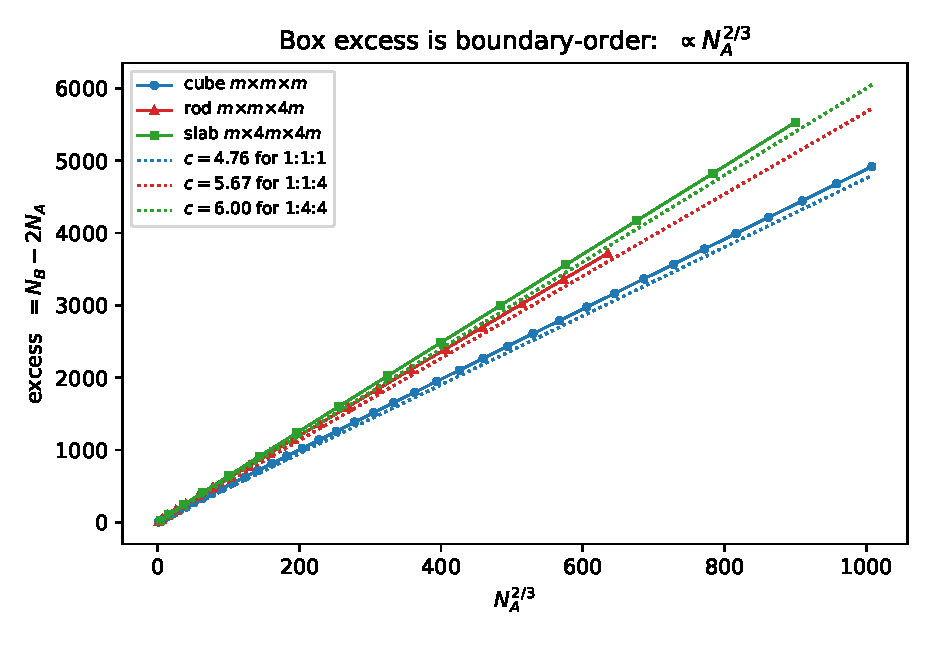
\includegraphics[width=0.82\linewidth]{figures/excess_vs_NA.pdf}}
  {\fbox{\parbox{0.7\linewidth}{\centering\itshape figure excess\_vs\_NA.pdf\\
   (run \texttt{scripts/plot\_ratio.py} to generate)}}}
\caption{For fixed axis-aligned aspect ratios, the excess $\NB-2\NA$ is a
boundary-order term proportional to $\NA^{2/3}$ to leading order.}
\end{figure}

\end{document}